\chapter{Cryptography and Cybersecurity Aspects} \label{ch:security}

Cryptography and cybersecurity serve as vital elements in a digital identity management system, in particular, in the decentralized systems of \gls{ssi},
which are based on blockchain. Cryptography enables the data to be tamper-proof, secure and privately shared through mechanisms such as hashing and digital signatures. This 
chapter explains the role of cryptography in \gls{ssi} while providing steps on how to create and verify integrity proofs, also, we demonstrate a digital signature 
algorithm implementation of \gls{eddsa}.

As mentioned earlier, cybersecurity also plays a key role in protecting \gls{ssi} systems from various threats and vulnerabilities. In this chapter we will highlight how, despite 
the inherent security features of blockchain technology, \gls{ssi} models still face several security challenges. Once this is done, potential attacks on \gls{ssi} systems, which arise 
precisely from these vulnerabilities, will be evaluated.

\section{Cryptography behind SSI}

\subsection{Data Integrity in SSI}

Among numerous cryptographic aspects in the \gls{ssi} approach, one of the most significant is perhaps the concept of proof used to verify the integrity and authenticity of VCs 
within the trust triangle, which forms the core of the \gls{ssi} model. In the rest of this subsection, we delve into how a proof is created, verified, and what are the parts 
that make it up.

\subsubsection{Proof Creation and Verification}

The essential steps for creating a data integrity proof in an \gls{ssi} system entail \cite{VCDataIntegrity}: 

\begin{enumerate}
  \item \textbf{Transformation}: This initial step entails the preparation of data inputs through converting them using canonicalization algorithms and binary-to-text encoding.
  \item \textbf{Hashing}: Cryptographic hash factories, for instance SHA-3, BLAKE-3 etc., provides hash identifiers that are resistant against hash collision and hence 
  ensure integrity and safety of data.
  \item \textbf{Proof Generation}: Implementing the proof serialization algorithms the values are calculated to make the input data secure from any inadmissible change. 
  Well-known examples are, digital signature and proofs of participation.
\end{enumerate}

\begin{figure}[h]  
  \centering
  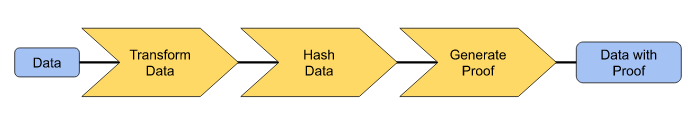
\includegraphics[width=1\textwidth]{Images/c5_1.png} 
  \caption{Process to create a cryptographic proof.}
\end{figure}

Next, verifying the proof requires three steps to be completed \cite{VCDataIntegrity}. The initial steps comprise the Transformation and Hashing processes which were previously presented, 
followed by the Cryptographic Proof Verification which involves some specific algorithms that confirm the reliability of the data being put in. It could mean checking up 
on the validity of digital signatures or verifying participation proofs.

\begin{figure}[h]  
  \centering
  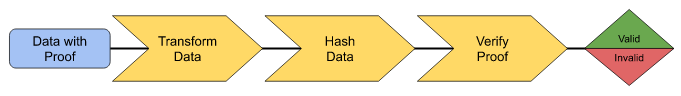
\includegraphics[width=1\textwidth]{Images/c5_2.png} 
  \caption{Process to verify a cryptographic proof.}
\end{figure}

\subsubsection{Proof Data Model}

A data integrity proof in \gls{ssi} systems consists of a number of parameters, some mandatory and some optional; among the first ones there are \cite{VCDataIntegrity}: 

\begin{itemize}
  \item \textbf{Type}: Identifies the exact proof type for cryptographic proof, thus, allows the relevant fields that are used to validate and verify the provided proof.
  \item \textbf{Proof Purpose}: Explicates the purpose of the proof, protects against the misuse and guarantees its proper implementation.
  \item \textbf{Verification Method}: Provides a description of the procedure and the data that may be required to verify the proof, which may involve cryptographic proofs 
  or other verification tools.
  \item \textbf{Proof Value}: It contains the encoded binary data that is required for proof verification, which is the process that uses the specific verification method.
\end{itemize}

\begin{figure}[h]  
  \centering
  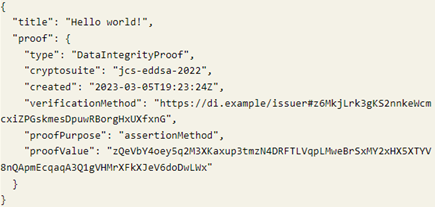
\includegraphics[width=0.8\textwidth]{Images/c5_3.png} 
  \caption{A simple example of cryptographic proof.}
\end{figure}

In addition, other optional parameters can also be included within a proof, such as \cite{VCDataIntegrity}: id, created, expires, domain (useful for representing the security domains in which the 
proof is meant to be used, ensuring its proper application within specified contexts) ,challenge (only if the domain is specific, to mitigate replay attacks), previousProof 
and nonce (useful to increase privacy by decreasing linkability, that is the result of deterministically generated signatures).

\subsection{Digital Signature using EdDSA}

In the manner before, the usage of the approach of digital signature is very common on the way of creating a proof. As a part of different algorithms, one that has the most 
outstanding impact is \gls{eddsa}, which its implementation we will cover in this subsection. Using the elliptic curve cryptography, the \gls{eddsa} is one of the most known for its 
speed and security.

\subsubsection{EdDSA Key Generation}

Key generation in \gls{eddsa} consists in the creation of a private-public key pair. The private key ($priKey$) consists of 32 octets of cryptographically secure random data 
(256 bit). For the public key ($pubKey$) the hashing algorithm (SHA-512) is applied to the private key as the first step in the process. And finally, the hashing product is 
converted using specific bit operations, as well as scalar multiplication, in order to get the public key \cite{10054286}. Specifically, this process involves the following steps:

\begin{enumerate}
  \item \textbf{Hashing}: The first step is hashing the private key (priKey) of 32-byte, using SHA-512, and store the result in a 64-octet buffer denoted as $h'$; only the 
  first 32-byte will be considered for the $pubKey$.
  \item \textbf{Buffer Pruning}: Then, some bit manipulations are performed on the buffer to ensure compliance with specific encoding requirements, for example some specific
  bits are clear in the first and last octets.
  \item \textbf{Scalar Multiplication}: The pruned buffer is then considered as a secret scalar represented by a little-endian integer and a fixed-base scalar multiplication
  $[s']B$ is performed, where $B$ represents a base point on the elliptic curve. 
  \item \textbf{Encoding}: Finally, the resulting point $[s']$ is encoded, through manipulation of the $y$-coordinate values of the curve. In this way the $pubKey$ has also 
  been generated.
\end{enumerate}

\subsubsection{EdDSA Signing}

Signatures are formed by using the private key to sign the message. This process is based on combining the message and the private key by using different cryptographic 
operations \cite{10054286}. In our case, the message corresponds to the value of the proof to be signed. Specifically, this process involves the following steps:

\begin{enumerate}
  \item \textbf{Hashing and Scalar Derivation}: The private key ($priKey$) is hashed using SHA-512 to obtain a digest ($h'$), of which the first half is used to create the 
  secret scalar $s'$, while the second half is denoted as prefix.
  \item \textbf{Message Hashing}: The message ($M'$) is hashed using SHA-512, along with prefix, context information ($CTX$) and a flag ($FLG$), so as to obtain a 64-octet 
  digest ($i$).
  \item \textbf{Point Calculation}: The point $[i]B$ is calculated, where $B$ is the base point on the elliptic curve. This calculation includes the reduction of 
  $i$ modulo $L$, that is, the group order of $B$, and finally the result is encoded, obtaining $R$.
  \item \textbf{Digest Calculation}: Then, another digest is computed by hashing the concatenation of $CTX$, $FLG$, $R$, the public key ($A$), and a modified hash of the message 
  ($PH(M')$), and from this is obtained the little-endian integer $k$.
  \item \textbf{Scalar Calculation}: $S' = (i + k \cdot s') \mod L$ is calculated.
  \item \textbf{Signature Construction}: Finally, the signature is created by concatenating $R$ (32 octets) and $S'$ (32 octets, with the three most significant bits at $0$) 
  in little-endian encoding.
\end{enumerate}

\subsubsection{EdDSA Verify Signature}

Signature verification attests to the authenticity of a certain signature by utilizing the public key, message (in our case the proof), and signature data. This method is 
based on decoding the signature, forming a digest out of the message and public key, and finally, verifying the group equation to ensure the integrity of the signature \cite{10054286}. 
Specifically, this process involves the following steps:

\begin{enumerate}
  \item \textbf{Signature Decoding}: Using the public key $A$ as reference point, the signature is decoded into two 32-octet parts, which represent the point $R$ and integer 
  $S'$, respectively.
  \item \textbf{Digest Generation}: Then, a 64-octet digest is generated by hashing the concatenation of $CTX$, $FLG$, $R$, public key ($A$), and a modified hash of the message 
  ($PH(M')$).
  \item \textbf{Group Equation Verification}: Finally, the validity of the signature is verified by checking the group equation $[8][S']B = [8]R + [8][k]A'$, or 
  alternatively, $[S']B = R + [k]A'$; where $A'$ is the public key encoded.
\end{enumerate}

\section{Cybersecurity within SSI}

\subsection{Security in Blockchain and SSI}

As previously outlined, in the context of \gls{ssi}, blockchain may be used as a distributed ledger to implement certain security features for the system. Nevertheless, this 
might not be sufficient enough because the \gls{ssi} model still contains some vulnerabilities. Next, we present the main features of blockchain technology, useful for the \gls{ssi} 
system, and after that we examine the security challenges according to the security assessment of the \gls{ssi} system. 

\subsubsection{Security Features in Blockchain}

Among the key security features of blockchain, those most crucial for decentralized identity management include \cite{CyberSecurity}:

\begin{itemize}
  \item \textbf{Tamper Resistance}: Data immutability is ensured via blockchain thus cryptographic hashing methods, linking each block cryptographically. Consensus 
  Protocols like Nakamoto consensus and digital signature algorithms such as \gls{ecdsa} mitigate the tampering of data.
  \item \textbf{DDoS Resistance}: The decentralized architecture of blockchains consensus protocols allows the reduction of DDoS attacks' impact, since they permit 
  transaction processing even with offline network nodes. In this scenario, attackers must compromise a significant portion of the network to make it inoperable.
  \item \textbf{Double Spending Resistance}: Consensus protocols and transparent transactions permit the mitigation of double-spending attacks, while verification 
  mechanisms guarantee transaction's validity, maintaining network integrity.
  \item \textbf{\%51 Resistance}: Attacks made against consensus protocols require the attacker to gain majority control, threatening the integrity of the transaction 
  history. Various consensus protocols have different susceptibility thresholds, so several robust security measures must be developed.
\end{itemize}

\subsubsection{Security Assessment of SSI}

The main challenges that \gls{ssi} models must approach are \cite{CyberSecurity}:

\begin{itemize}
  \item \textbf{Dependency on Manufacturer Reliability}: \gls{ssi} systems depend on \gls{tee}s supplied by the manufacturers, which is crucial for 
  the security of the systems. The reliance put on the security model manufacturers come up with is also dubious and might introduce further vulnerabilities associated with 
  single points of failure.
  \item \textbf{Data Availability and Memory Risks}: Storing verifiable credentials in a local storage in the \gls{ssi} systems can decrease the accessibility and can expose 
  issues related to memory corruption or misuse. The availability of the data spot on without ruining the integrity is a big question.
  \item \textbf{Confidentiality Protection and Information Disclosure Risks}: Although \gls{ssi} systems are using different methods such as anonymous authentication and 
  \gls{zkp}s to protect privacy, risks for disclosing sensitive identity information still remain. The reasonable selective disclosure mechanisms are 
  still under development. The implementation of these mechanisms should be improved to mitigate the risks.
\end{itemize}

\subsection{Potential Attacks on the SSI System}

The vulnerabilities identified in the previous segment could give malicious actors the push to conduct different types of attacks and lead to damage or steal identities of other 
people to the \gls{ssi} system. These attacks can be grouped into three categories, and an attack tree can be defined for each of them in order to better analyze them.

\subsubsection{Fake Identity Attacks}

Fake identity attacks pose a major threat to \gls{ssi} systems, using fake identities to gain access to services they are not authorized for. Attackers exploit vulnerabilities in 
the \gls{ssi} architecture to create fake credentials. These attacks can damage the trust and reliability of the identity management system as a whole \cite{CyberSecurity}.

\begin{figure}[h]  
  \centering
  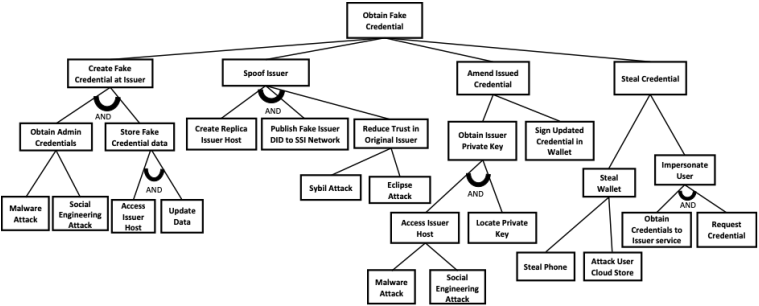
\includegraphics[width=1\textwidth]{Images/c5_4.png} 
  \caption{An attack tree of Faking Identity Attacks in the SSI system.}
\end{figure}

\newpage

\textbf{Attack Tree Analysis}: In this attack scenario, attackers pretend to be trusted issuers by creating fake credentials, like \gls{did}s and public keys. Once inside the 
network, they trick it into believing these fake credentials are real. In addiction, vulnerabilities in the architecture, like hacked network machines, can give attackers 
access to secret administrative credentials and keys, allowing them to change them. For instance, in the Eclipse Attack, attackers take control of the peer-to-peer network 
by redirecting connections to fake nodes, making the network accept the false credentials \cite{9659929}.

\subsubsection{Identity Theft Attacks}

Identity theft attacks use vulnerabilities, in the \gls{ssi} system to steal sensitive and personal information, from user wallets without permission. These actions put 
individuals’ privacy at risk and could result in types of fraudulent activities and improper use of personal data \cite{CyberSecurity}. 

\begin{figure}[h]  
  \centering
  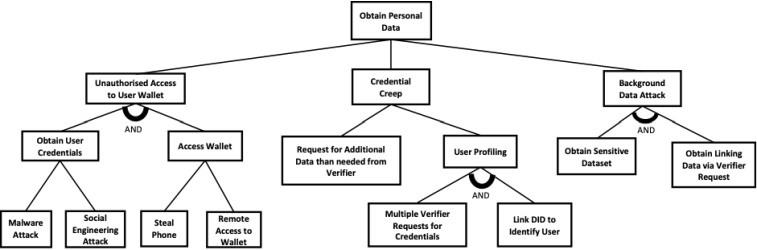
\includegraphics[width=1\textwidth]{Images/c5_5.png} 
  \caption{An attack tree of Theft Identity Attacks in the SSI system.}
\end{figure}

\textbf{Attack Tree Analysis}: In this type of attack, malicious actors might access data in wallets without permission by exploiting vulnerabilities in the \gls{ssi} 
infrastructure. To do that, They could exploit authentication weaknesses or misuse credential verification methods to obtain additional personal information, a practice 
known as Credential Creep. The impact of identity theft attacks goes beyond users impacting the credibility and reliability of the \gls{ssi} environment as a whole \cite{9659929}. 

\subsubsection{DDoS Attacks}

\gls{ddos} attacks pose a serious risk to the availability and reliability of \gls{ssi} system services. Through attacking the system with a large 
volume of traffic, the attackers intend to cripple the users’ access to the system and breach the system’s function \cite{CyberSecurity}.

\begin{figure}[h]  
  \centering
  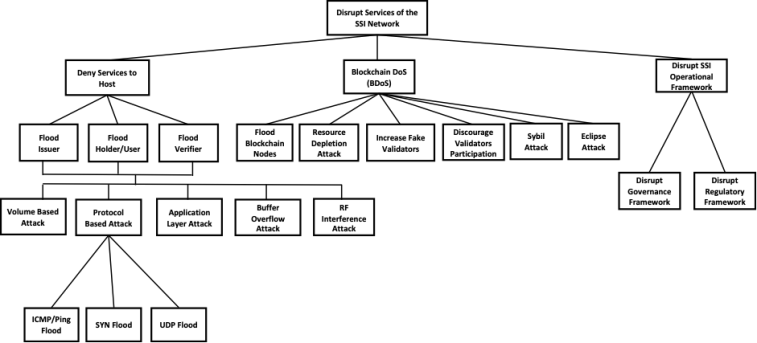
\includegraphics[width=1\textwidth]{Images/c5_6.png} 
  \caption{An attack tree of Distributed DDoS Attacks in the SSI system.}
\end{figure}

\textbf{Attack Tree Analysis}: This type of attacks aim at several parts of the \gls{ssi} system, such as issuer, holder, and verifier hosts, along with the distributed ledger nodes. 
Malicious actors can exploit vulnerabilities to attacks using vulnerabilities in the blockchain infrastructure, for example flooding the nodes or disrupting the consensus 
process. Furthermore, operational frameworks can be targeted, leading to difficulties in governance and regulatory processes that are imperative for the functioning of the 
\gls{ssi} ecosystem \cite{9659929}.